%!TEX program = pdflatex
% ============================================================
%  Presentación Beamer — TFG V3 (Estilo Limpio y Exhaustivo)
% ============================================================
\documentclass[aspectratio=169, 12pt]{beamer}

\usepackage[T1]{fontenc}
\usepackage[utf8]{inputenc}
\usepackage[spanish, es-noshorthands]{babel}
\usepackage[mono=false]{libertine}

\usepackage{graphicx}
\graphicspath{{../TFG_PDF_LATEX_PROJECT/}, {.}}
\usepackage{tikz}
\usetikzlibrary{arrows.meta, positioning, calc, shapes.geometric, backgrounds, fit}

\usepackage{amsmath, amssymb, bm}
\usepackage{csquotes}
\usepackage[backend=biber, style=authoryear, maxcitenames=2, uniquelist=false, doi=false, isbn=false, url=false]{biblatex}
\addbibresource{../TFG_PDF_LATEX_PROJECT/referencias.bib}

% ============================================================
% Ajuste de Bibliografía a pie de página
% ============================================================
\setbeamerfont{footnote}{size=\tiny}
\renewcommand{\footnotesize}{\tiny}

% ============================================================
%  COLORES CORPORATIVOS — Universidad de Sevilla
% ============================================================
\definecolor{USred}{cmyk}{0,1.00,0.65,0.34}
\definecolor{USlight}{RGB}{245,235,235}
\definecolor{Black}{RGB}{0,0,0}

% ============================================================
%  TEMA BEAMER PERSONALIZADO LIMPIO
% ============================================================
\usetheme{default}
\usecolortheme{default}

\setbeamercolor{structure}{fg=USred}
\setbeamercolor{title}{fg=Black}
\setbeamercolor{frametitle}{fg=USred, bg=white}
\setbeamerfont{frametitle}{series=\bfseries, size=\large}
\setbeamercolor{item}{fg=USred}
\setbeamercolor{subitem}{fg=USred!70}

% Limpiar bloques de color, todo a texto plano excepto el título
\setbeamercolor{block title}{fg=Black, bg=white}
\setbeamercolor{block body}{bg=white}
\setbeamercolor{block title alerted}{fg=USred, bg=white}
\setbeamercolor{block body alerted}{bg=white}

% Cabecera limpia sin logo
\setbeamertemplate{headline}{}

% Footline ajustado para que la paginación no se salga
\setbeamercolor{author in head/foot}{bg=USred, fg=white}
\setbeamercolor{title in head/foot}{bg=USred!85!black, fg=white}
\setbeamercolor{page in head/foot}{bg=USred!70!black, fg=white}

\setbeamertemplate{footline}{%
  \leavevmode%
  \hbox{%
    \begin{beamercolorbox}[wd=.33\paperwidth,ht=2.5ex,dp=1.2ex,leftskip=.3cm]{author in head/foot}%
      \usebeamerfont{author in head/foot}\insertshortauthor
    \end{beamercolorbox}%
    \begin{beamercolorbox}[wd=.34\paperwidth,ht=2.5ex,dp=1.2ex,center]{title in head/foot}%
      \usebeamerfont{title in head/foot}\insertshorttitle
    \end{beamercolorbox}%
    \begin{beamercolorbox}[wd=.33\paperwidth,ht=2.5ex,dp=1.2ex,rightskip=.3cm,right]{page in head/foot}%
      \insertframenumber\,/\,\inserttotalframenumber
    \end{beamercolorbox}%
  }%
  \vskip0pt%
}
\setbeamertemplate{navigation symbols}{}

% Transiciones de sección
\AtBeginSection[]{
  \begin{frame}[plain]
    \vfill
    \centering
    {\LARGE\bfseries \color{USred} \insertsectionhead\par}
    \vfill
  \end{frame}
}

% ============================================================
%  DATOS DEL DOCUMENTO
% ============================================================
\title{Fundamentos Matemáticos de los\\Energy-Based Models y las\\Joint Embedding Architectures}
\author[P. Rivas Vega]{Pedro Rivas Vega}
\institute{Grado en Matemáticas — Universidad de Sevilla}
\date{Julio 2026}
\titlegraphic{
\includegraphics[height=2cm]{sello.pdf}}

\begin{document}

\begin{frame}[plain]
\titlepage
\end{frame}

\begin{frame}{Cronología}
\centering
\vspace{0.3cm}
\resizebox{0.95\linewidth}{!}{%
\begin{tikzpicture}[
    >=Stealth,
    timeline/.style={ultra thick, ->, draw=gray!50},
    mathnode/.style={circle, fill=blue!15, draw=blue!80!black, thick, inner sep=2pt, minimum size=8pt},
    jeanode/.style={circle, fill=orange!15, draw=orange!80!black, thick, inner sep=2pt, minimum size=8pt},
    yearmath/.style={above, font=\scriptsize\bfseries, text=blue!80!black, yshift=4pt},
    descmath/.style={below, font=\scriptsize, align=center, text width=2.4cm, yshift=-4pt},
    yearjea/.style={above, font=\scriptsize\bfseries, text=orange!80!black, yshift=4pt},
    descjea/.style={below, font=\scriptsize, align=center, text width=2.2cm, yshift=-4pt},
    titlebox/.style={font=\normalsize\bfseries, align=left}
]

  % --- Línea Superior: Resultados Matemáticos Clásicos ---
  \node[titlebox, text=blue!80!black, anchor=west] at (-1.5, 2.5) {Hitos Matemáticos Fundamentales};
  \draw[timeline] (-1.5, 1) -- (16.5, 1);
  
  \foreach \x/\yr/\desc in {
    0.5/1936/Teorema de\\Cramér-Wold, 
    5.0/1957/Principio de\\Jaynes, 
    10.0/1961/Reducción de\\Redundancia (Barlow), 
    15.0/1983/Test Diferenciable\\(Epps-Pulley)%
  }{
    \node[mathnode] (m\yr) at (\x, 1) {};
    \node[yearmath] at (m\yr.north) {\yr};
    \node[descmath] at (m\yr.south) {\desc};
  }

  % --- Línea Inferior: Evolución de las JEA ---
  \node[titlebox, text=orange!80!black, anchor=west] at (-1.5, -1.5) {Evolución de las Joint Embedding Architectures (JEA)};
  \draw[timeline] (-1.5, -3) -- (16.5, -3);

  \foreach \x/\yr/\desc in {
    0.0/1993/Redes\\Siamesas, 
    2.5/2006/Contrastive\\Learning, 
    5.0/2020/BYOL, 
    7.0/2021/Barlow\\Twins,
    9.2/2022/VICReg\\PLDM, 
    11.4/2023/V-JEPA, 
    13.6/2025/SIGReg, 
    15.8/2026/Garantías\\(Klindt)%
  }{
    \node[jeanode] (j\yr) at (\x, -3) {};
    \node[yearjea] at (j\yr.north) {\yr};
    \node[descjea] at (j\yr.south) {\desc};
  }

\end{tikzpicture}%
}
\end{frame}

% ────────────────────────────────────────────────────────────
\section{Capítulo 1: Introducción y Paradigma JEA}

\begin{frame}{El papel de la observación en el aprendizaje}
La mayor parte del conocimiento se adquiere por observación pura de datos continuos (imágenes, vídeo), sin supervisión externa. 

Las etiquetas humanas son un porcentaje mínimo de la información que procesa un agente inteligente.\footcite{lecun2022path}

Los grandes modelos de lenguaje (LLM) han resuelto este aprendizaje autosupervisado (SSL) en dominios discretos. El objetivo de este trabajo es entender su traslación matemática al mundo continuo.
\end{frame}

\begin{frame}{Paradigma Discriminativo y Generativo}
Los dos enfoques clásicos del aprendizaje automático presentan limitaciones estructurales para capturar abstracciones en alta dimensión:
\vspace{0.5cm}
\begin{itemize}
    \item \textbf{Modelos Discriminativos ($x \to y$):} Requieren un oráculo (etiquetas humanas) y descartan sistemáticamente información de la entrada.
    \item \textbf{Modelos Generativos ($x \to \hat{x}$):} Se ven obligados a invertir capacidad de red en reconstruir detalles estocásticos impredecibles a nivel de píxel (p.e. las hojas de un árbol moviéndose por el viento).
\end{itemize}
\end{frame}

\begin{frame}{Joint Embedding Architectures (JEA)}
Las JEA abordan el problema operando exclusivamente en un espacio latente abstracto $\mathcal{Z}$. 

\vspace{0.5cm}
En lugar de generar o reconstruir la entrada, el modelo proyecta dos entradas relacionadas ($x, y$) a un espacio comprimido de características ($z_x, z_y$) y evalúa la similitud matemática entre sus representaciones.

Esto permite al modelo ignorar información irrelevante y retener solo el núcleo semántico.
\end{frame}

\begin{frame}{Arquitectura Conceptual JEA}
\centering
\resizebox{0.75\linewidth}{!}{%
\begin{tikzpicture}[node distance=1.5cm, auto, >=Stealth]
    \node (x) [draw, rectangle, minimum width=2.5cm, minimum height=1cm] {Entrada $x$};
    \node (y) [draw, rectangle, minimum width=2.5cm, minimum height=1cm, below=of x] {Entrada $y$};
    \node (fx) [draw, rectangle, minimum width=2cm, minimum height=1cm, right=of x, xshift=1cm] {Encoder $f_{\theta}$};
    \node (gy) [draw, rectangle, minimum width=2cm, minimum height=1cm, right=of y, xshift=1cm] {Encoder $g_{\phi}$};
    \node (zx) [circle, draw, right=of fx, xshift=1cm] {$z_x$};
    \node (zy) [circle, draw, right=of gy, xshift=1cm] {$z_y$};
    \node (loss) [draw, diamond, minimum width=1.5cm, minimum height=1.5cm, right=of zx, yshift=-1.1cm, xshift=1cm] {Loss}; 
    \draw[->] (x) -- (fx);
    \draw[->] (y) -- (gy);
    \draw[->] (fx) -- (zx);
    \draw[->] (gy) -- (zy);
    \draw[->] (zx) -| (loss);
    \draw[->] (zy) -| (loss);
    \draw[dashed, <->] (fx) -- node[left] {Shared $\theta$ (opcional)} (gy);
\end{tikzpicture}%
}
\end{frame}

% ────────────────────────────────────────────────────────────
\section{Capítulo 2: Modelos Basados en Energía}

\begin{frame}{La Función de Energía (1/2)}
Las JEA se formalizan mediante los Modelos Basados en Energía (EBM).\footcite{lecun2006tutorial}

Un EBM asigna un valor escalar (energía) a cada configuración de variables $(x, y)$, que cuantifica su grado de \textbf{incompatibilidad}:
\[
    E_\theta : \mathcal{X} \times \mathcal{Y} \to \mathbb{R}
\]

En las arquitecturas Joint Embedding, la energía es típicamente la distancia euclídea al cuadrado en el espacio latente:
\[
    E_\theta(x, y) = \|f_\theta(x) - g_\phi(y)\|_2^2
\]
\end{frame}

\begin{frame}{La Función de Energía (2/2)}
A diferencia de los modelos probabilísticos, la integral de la superficie de energía sobre el espacio de variables no tiene por qué sumar uno.

La inferencia se reduce a un problema de optimización continuo, buscando el estado fundamental o de mínima energía:
\[
    y^* = \arg\min_{y \in \mathcal{Y}} E_\theta(x, y)
\]
\end{frame}

\begin{frame}{El Principio de Máxima Entropía de Jaynes (1/2)}
Si se desea convertir la energía en una probabilidad, la formulación matemática correcta es la Medida de Boltzmann-Gibbs:
\[
    p_\theta(y | x) = \frac{e^{-\beta E_\theta(x, y)}}{Z(x; \theta)}
\]

Edwin T. Jaynes (1957) demostró formalmente por qué esta es la elección canónica: es la única distribución probabilística que maximiza la Entropía de Shannon sujeta a un valor esperado de energía.\footcite{jaynes1957information}
\end{frame}

\begin{frame}{El Principio de Máxima Entropía de Jaynes (2/2)}
El término $Z(x; \theta)$ es la función de partición. Se encarga de normalizar la distribución integrando (o sumando) la energía sobre todo el dominio posible de la variable $y$:
\[
    Z(x; \theta) = \int_{y \in \mathcal{Y}} e^{-\beta E_\theta(x, y)} \, dy
\]
\end{frame}

\begin{frame}{El cuello de botella probabilístico}
El cálculo de la función de partición es la barrera infranqueable del aprendizaje continuo.

\begin{itemize}
    \item \textbf{Dominio discreto (LLMs):} $\mathcal{Y}$ es un vocabulario finito ($10^5$ palabras). La integral se convierte en un sumatorio tratable, conocido como la función \textit{Softmax}.
    \item \textbf{Dominio continuo (Visión):} $\mathcal{Y}$ es un espacio vectorial masivo (imágenes). La integral es intratable analítica y numéricamente.
\end{itemize}
\vspace{0.5cm}
Por este motivo, las JEA abandonan el marco probabilístico de Boltzmann y se ven forzadas a optimizar la energía escalar sin normalizar.
\end{frame}

% ────────────────────────────────────────────────────────────
\section{Capítulo 3: Redes Siamesas y el Colapso}

\begin{frame}{Redes Siamesas (1993)}
El abandono de la función de partición provoca el problema central de toda esta familia de modelos: el colapso de representación.

Bromley y LeCun (1993) propusieron la primera JEA, las Redes Siamesas, usando una única función de pérdida positiva que aproxima las representaciones de vistas relacionadas:\footcite{bromley1993signature}
\[
    \mathcal{L}_{\text{pos}}(W) = \mathbb{E}_{(x_1, x_2) \sim p_{\text{pos}}} \left[ \| f_W(x_1) - f_W(x_2) \|_2^2 \right]
\]
\end{frame}

\begin{frame}{El Colapso Constante como Mínimo Global}
\textbf{Teorema:}
Cualquier mapeo constante de la forma $f_{W^*}(x) = c$ para todo $x$, donde $c \in \mathbb{R}^d$ es un vector constante arbitrario, es un mínimo global absoluto de la pérdida $\mathcal{L}_{\text{pos}}(W)$.

\vspace{0.5cm}
\textbf{Prueba directa:}
Por definición de norma euclídea: $\|f_W(x_1) - f_W(x_2)\|_2^2 \geq 0$.
Si $f(x)=c$ para todo $x$, entonces la distancia es $\|c - c\|_2^2 = 0$. Como la cota inferior es $0$, se trata de un mínimo global. El gradiente es exactamente cero, por lo que el estado de colapso es un atractor estable del que el optimizador no puede escapar.
\end{frame}

\begin{frame}{Visualización del Colapso Siamés}
\centering
\resizebox{0.75\linewidth}{!}{%
\begin{tikzpicture}[node distance=1.5cm, auto, >=Stealth]
    \node (x1) [draw, rectangle, minimum width=2.5cm, minimum height=1.5cm] {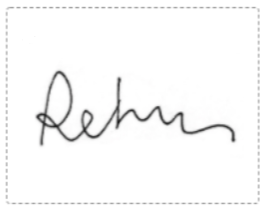
\includegraphics[width=2.3cm, height=1.3cm]{signature_Rodlf1.png}};
    \node (x2) [draw, rectangle, minimum width=2.5cm, minimum height=1.5cm, below=of x1, yshift=-0.5cm] {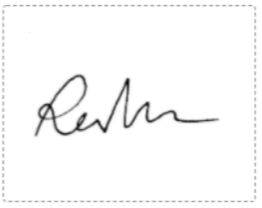
\includegraphics[width=2.3cm, height=1.3cm]{signature_Rodlf2.png}};
    \node [above=0.05cm of x1, font=\footnotesize] {Entrada $x_1$ (Firma A)};
    \node [below=0.05cm of x2, font=\footnotesize] {Entrada $x_2$ (Firma B)};
    \node (f1) [draw, rectangle, minimum width=2cm, minimum height=1cm, right=of x1, xshift=1cm] {Encoder $f_{W}$};
    \node (f2) [draw, rectangle, minimum width=2cm, minimum height=1cm, right=of x2, xshift=1cm] {Encoder $f_{W}$};
    \node (z) [circle, draw, double, red, thick, minimum size=1.5cm] at ($(f1.east)!0.5!(f2.east) + (2.5cm,0)$) {$z_1 = z_2 = c$};
    \node [above=0.1cm of z, font=\footnotesize\bfseries, align=center, red] {Espacio Latente $\mathcal{Z}$\\};
    \node (loss) [draw, diamond, minimum width=1.5cm, minimum height=1.5cm, right=of z, xshift=0cm] {Loss = 0}; 
    \draw[->] (x1) -- (f1); \draw[->] (x2) -- (f2);
    \draw[->] (f1.east) -- (z.north west); \draw[->] (f2.east) -- (z.south west);
    \draw[->] (z) -- (loss);
    \draw[dashed, <->] (f1) -- node[left] {Shared $W$} (f2);
\end{tikzpicture}%
}
\end{frame}

\begin{frame}{Colapso Dimensional}
Incluso si el modelo evade el colapso constante, es vulnerable al colapso dimensional: las características se contraen ocupando un subespacio lineal de rango muy inferior a la dimensión teórica $d$.

\vspace{0.5cm}
\textbf{Dinámica de flujo de gradiente:}
El término $\|f(x_1) - f(x_2)\|_2^2$ somete a cada componente de los pesos a una fuerza de decaimiento continuo. Como demostraron Jing et al. (2022),\footcite{jing2022understanding} cada dimensión del espacio decae exponencialmente a una tasa que depende de la varianza en esa dirección.
\end{frame}

% ────────────────────────────────────────────────────────────
\section{Capítulo 4: Contrastive Learning}

\begin{frame}{Pérdida Contrastiva con Margen (1/2)}
La primera solución matemática al colapso fue la de Hadsell, Chopra y LeCun (2006).\footcite{hadsell2006dimensionality} Añadieron pares negativos (imágenes semánticamente distintas, $Y=0$) para crear una fuerza de repulsión.

\vspace{0.5cm}
Fórmula de la Pérdida Contrastiva:
\[
    \mathcal{L}_\text{cont}(W) = \frac{1}{2}\,\mathbb{E}\left[ Y\, d_W^2 + (1-Y)\max(0, m - d_W)^2 \right]
\]

Donde $d_W$ es la distancia euclídea y $m$ es el margen de seguridad.
\end{frame}

\begin{frame}{Pérdida Contrastiva con Margen (2/2)}
Al calcular el gradiente de un par negativo, si la distancia está dentro del margen $m$, la fuerza generada es:
\[
    \nabla_W \mathcal{L}_{\text{neg}} = -(m - d_W) \nabla_W d_W
\]
Este signo negativo garantiza que el optimizador \textbf{empuje} las representaciones alejándolas mutuamente, lo que impide que las proyecciones colapsen en un único punto geométrico.
\end{frame}

\begin{frame}{Dinámica de las Fuerzas Contrastivas}
\centering
\resizebox{0.95\linewidth}{!}{%
\begin{tikzpicture}[>=Stealth, node distance=2cm]
    % --- Fuerzas de Atracción (Positivos) ---
    \node[align=center, font=\small] (title_pos) at (-4, 2.2) {\textbf{Pares Positivos} ($Y=1$) \\ Atracción tipo Muelle};
    \node[circle, fill=blue!15, draw=blue, thick, minimum size=0.8cm] (p1) at (-5.4, 0) {$z_1$};
    \node[circle, fill=blue!15, draw=blue, thick, minimum size=0.8cm] (p2) at (-2.6, 0) {$z_2$};
    \draw[->, ultra thick, blue] (p1.east) -- ++(0.9, 0);
    \draw[->, ultra thick, blue] (p2.west) -- ++(-0.9, 0);
    \node[blue, font=\small\bfseries] at (-4, -2.2) {Atracción: $\mathbf{F} \propto d_W$};

    % --- Fuerzas de Repulsión (Negativos, d < m) ---
    \node[align=center, font=\small] (title_neg_in) at (1, 2.2) {\textbf{Pares Negativos} ($Y=0$) \\ Repulsión activa ($d_W < m$)};
    \node[circle, fill=red!15, draw=red, thick, minimum size=0.8cm] (n1_in) at (1, 0) {$z_1$};
    \draw[dashed, red, thick] (n1_in) circle (1.6cm);
    \draw[->, red, densely dotted] (n1_in.center) -- ++(-1.6, 0) node[midway, above, font=\footnotesize] {$m$};
    \node[circle, fill=red!15, draw=red, thick, minimum size=0.8cm] (n2_in) at (2.1, 0.7) {$z_2$};
    \draw[->, ultra thick, red] (n1_in) -- ++(-1.0, -0.7);
    \draw[->, ultra thick, red] (n2_in) -- ++(1.0, 0.7);
    \node[red, font=\small\bfseries] at (1, -2.0) {Repulsión ($\mathbf{F} > 0$)};

    % --- Sin Fuerzas (Negativos, d >= m) ---
    \node[align=center, font=\small] (title_neg_out) at (6, 2.2) {\textbf{Pares Negativos} ($Y=0$) \\ Reposo ($d_W \ge m$)};
    \node[circle, fill=gray!15, draw=gray, thick, minimum size=0.8cm] (n1_out) at (6, 0) {$z_1$};
    \node[circle, fill=gray!15, draw=gray, thick, minimum size=0.8cm] (n2_out) at (8.0, 0.8) {$z_2$};
    \draw[dashed, gray, thick] (n1_out) circle (1.6cm);
    \draw[->, gray, densely dotted] (n1_out.center) -- ++(-1.6, 0) node[midway, above, font=\footnotesize] {$m$};
    \node[gray, font=\small\bfseries] at (6, -2.0) {Reposo ($\mathbf{F} = 0$)};
\end{tikzpicture}%
}
\end{frame}

\begin{frame}{El límite de la Epsilon-Red}
Para que las pérdidas contrastivas prevengan el colapso dimensional, la repulsión debe aplicarse uniformente en todas las dimensiones de la hiperesfera $\mathbb{S}^{d-1}$.\footcite{vershynin2018high}

\vspace{0.5cm}
Por la teoría de Epsilon-Redes, el número mínimo de puntos (ejemplos negativos) necesarios para cubrir la superficie de una esfera dimensional con esferas de radio $\varepsilon$ (margen) crece como:
\[
    N(\mathbb{S}^{d-1}, \varepsilon) \approx \left( \frac{1}{\varepsilon} \right)^d
\]
Esta escala $\mathcal{O}(e^d)$ hace que el problema sea intratable en los grandes espacios del aprendizaje profundo.
\end{frame}

\begin{frame}{Visualización de Zonas Ciegas}
\centering
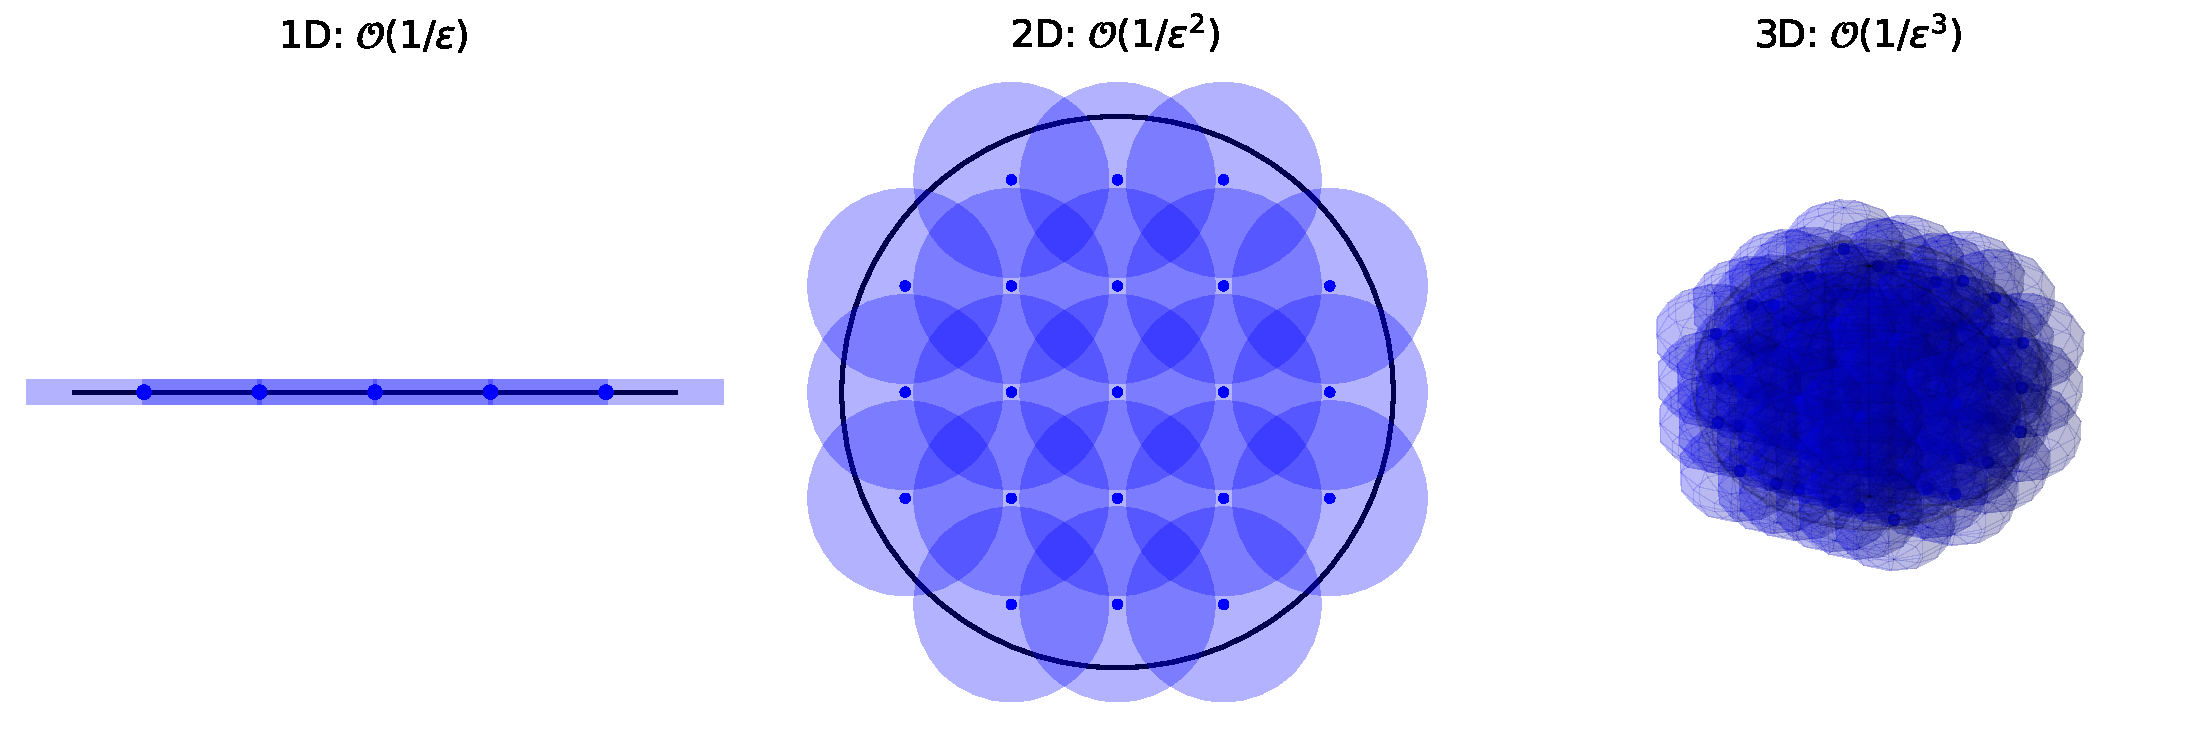
\includegraphics[width=0.95\linewidth, height=0.8\textheight, keepaspectratio]{epsilon_net.pdf}
\end{frame}

% ────────────────────────────────────────────────────────────
\section{Capítulo 5: Revolución No Contrastiva}

\begin{frame}{La Hipótesis de Barlow (1961)}
\begin{columns}
\begin{column}{0.75\textwidth}
Ante el límite exponencial de los negativos, se acude a la neurobiología. 

Horace Barlow postuló que el cerebro decodifica las señales sensoriales minimizando la redundancia entre neuronas.\footcite{barlow1961possible}

El objetivo es que las representaciones finales sean mutuamente \textbf{independientes}, de forma que la red no malgaste capacidad de canal en transmitir información predecible por el contexto.
\end{column}
\begin{column}{0.25\textwidth}
\centering
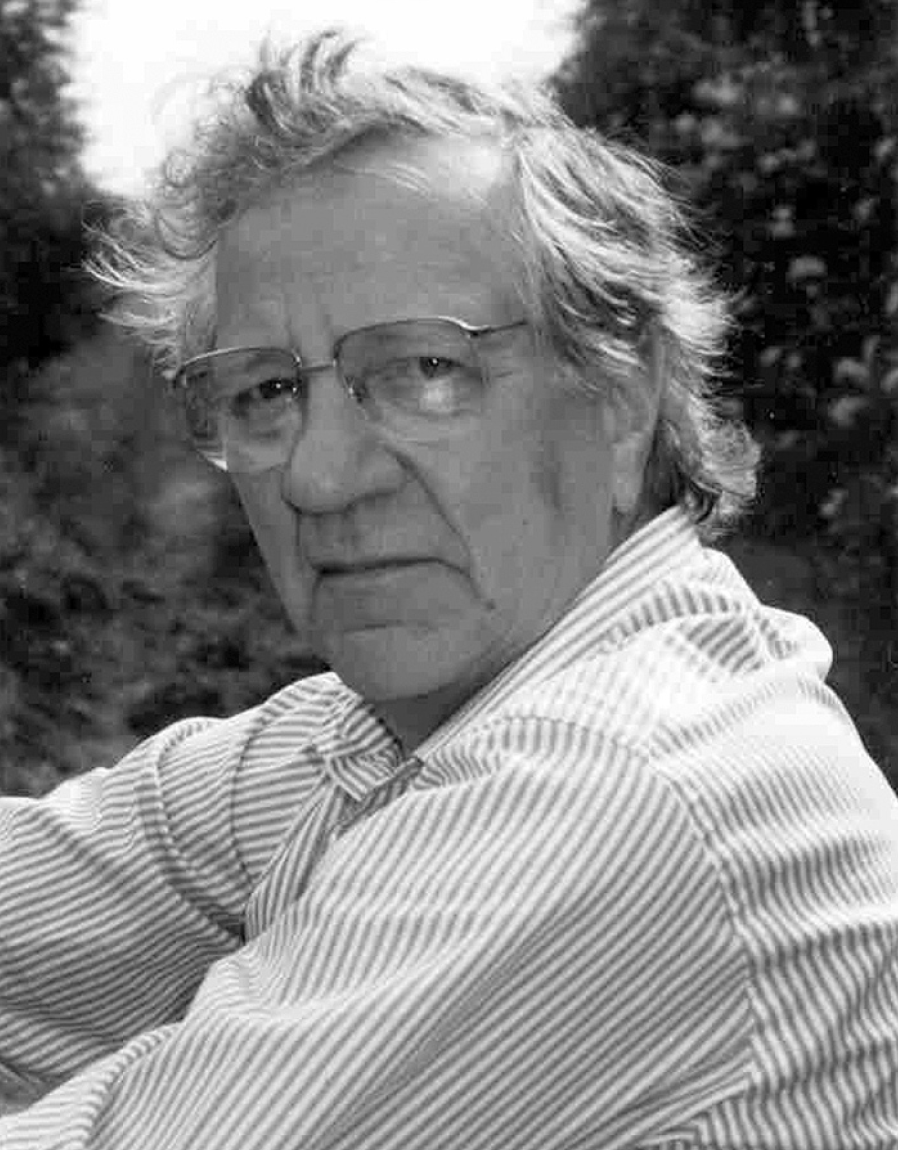
\includegraphics[width=\linewidth, keepaspectratio]{barlow.png}
\end{column}
\end{columns}
\end{frame}

\begin{frame}{Información Mutua y Entropía}
La independencia no puede medirse solo con la correlación lineal (que ignora dependencias no lineales). La métrica ideal es la \textbf{Información Mutua} de Shannon.\footcite{shannon1948mathematical}

La entropía individual $H(z_i)$ mide la información de una neurona. La información compartida por dos neuronas es:
\[
    I(z_i; z_j) = H(z_i) + H(z_j) - H(z_i, z_j)
\]
Si son independientes, $I(z_i; z_j) = 0$.
\end{frame}

\begin{frame}{Matriz de Información Mutua}
Para todo el vector latente, definimos la matriz $\mathcal{I}(Z) \in \mathbb{R}^{d \times d}$:
\[
    \mathcal{I}(Z)_{ij} = 
    \begin{cases}
    H(z_i) & \text{si } i = j \\
    I(z_i; z_j) & \text{si } i \neq j
    \end{cases}
\]

El objetivo ideal de Barlow equivale a forzar que $\mathcal{I}(Z)$ sea una \textbf{matriz diagonal}: máxima retención de información propia (evita colapso) y nula información compartida (independencia).
\end{frame}

\begin{frame}{Diagonalizar la Información Mutua}
\centering
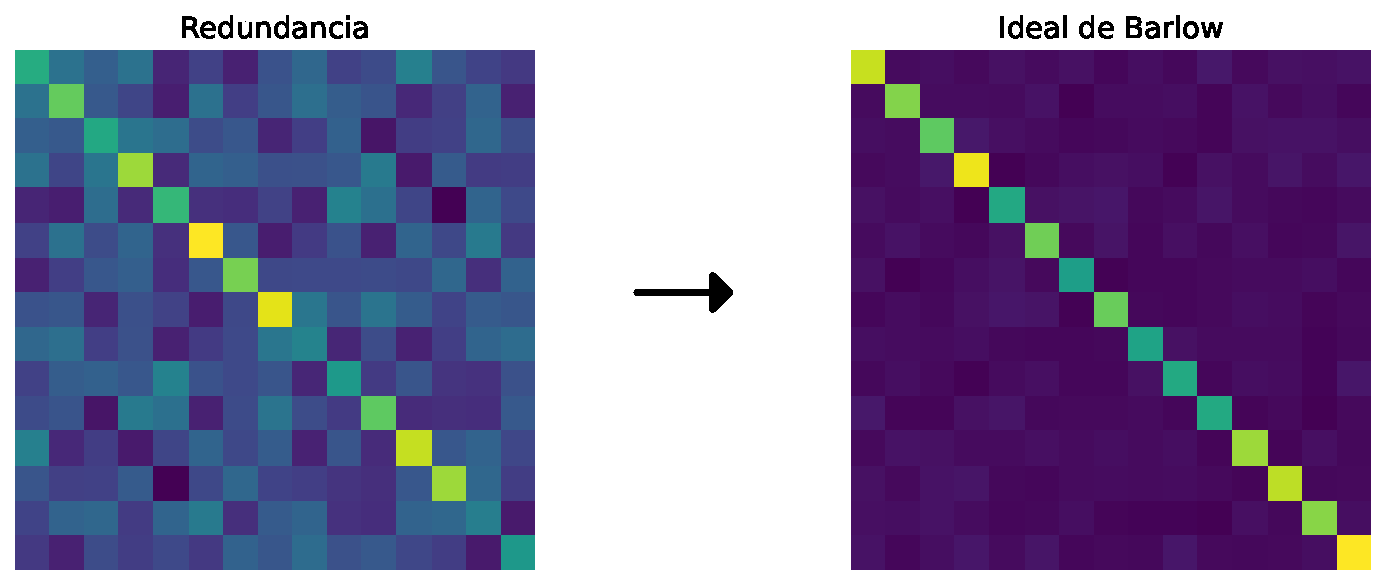
\includegraphics[width=0.95\linewidth, height=0.8\textheight, keepaspectratio]{heatmaps_IZ.pdf}\\[4pt]
\end{frame}

\begin{frame}{El Problema de la Intratabilidad}
Estimar $\mathcal{I}(Z)$ requiere conocer la función de densidad conjunta $p(Z)$ de los datos, lo cual es inobservable en problemas reales.

Además, su aproximación empírica sufre del mismo coste exponencial que el contrastive learning en dimensiones altas.
\end{frame}

\begin{frame}{El Puente de Jaynes}
La solución reside en una equivalencia fundamental. Si asumimos que las representaciones latentes $Z$ siguen una distribución \textbf{Gaussiana Multivariante}, la Información Mutua depende únicamente del coeficiente de correlación de Pearson $\rho_{ij}$:
\[
    I(z_i; z_j) = -\frac{1}{2} \log(1 - \rho_{ij}^2)
\]
Esta proposición indica que, bajo gaussianidad, la correlación lineal captura \emph{todas} las dependencias estadísticas.
\end{frame}

\begin{frame}{Equivalencia bajo Gaussianidad}
\textbf{Corolario:} Sea $R \in \mathbb{R}^{d \times d}$ la matriz de correlación de Pearson. Bajo la hipótesis de normalidad, garantizar la independencia es equivalente a imponer la decorrelación lineal:
\[
    \mathcal{I}(Z) \text{ es diagonal } \iff R = I_d
\]

\textbf{Demostración:}
Para $i \neq j$, queremos $I(z_i; z_j) = 0$.
\[
    -\frac{1}{2} \log(1 - \rho_{ij}^2) = 0 \iff 1 - \rho_{ij}^2 = 1 \iff \rho_{ij} = 0
\]
Como la diagonal de $R$ es siempre $1$, la condición equivale a $R = I_d$.
\end{frame}

\begin{frame}{Construcción en Barlow Twins}
Barlow Twins (2021) implementa este puente. Se generan dos vistas $x_1, x_2$, y se extraen los batches $Z^A, Z^B \in \mathbb{R}^{N \times d}$.\footcite{zbontar2021barlow}

Primero, se \textbf{centran en media} las columnas a lo largo del batch:
\[
    z_k^{A,(i)} \gets z_k^{A,(i)} - \frac{1}{N}\sum_{m=1}^N z_k^{A,(m)}
\]
Esto garantiza que se evalúe la verdadera covarianza, sin estar dominada por la magnitud de las medias.
\end{frame}

\begin{frame}{Matriz de Correlación Cruzada Empírica}
Se define la matriz empírica $C \in \mathbb{R}^{d \times d}$ calculando la similitud coseno entre las columnas de ambas vistas:
\[
    C_{kl} = \frac{\langle \mathbf{z}_k^A, \mathbf{z}_l^B \rangle}{\|\mathbf{z}_k^A\|_2 \, \|\mathbf{z}_l^B\|_2} = \frac{\sum_{i=1}^{N} z_k^{A,(i)} z_l^{B,(i)}}{\sqrt{\sum_{i=1}^{N} (z_k^{A,(i)})^2} \sqrt{\sum_{i=1}^{N} (z_l^{B,(i)})^2}}
\]
Por su normalización euclídea, $C_{kl} \in [-1, 1]$.
\end{frame}

\begin{frame}{La Pérdida de Barlow Twins}
La pérdida final penaliza la discrepancia de $C$ respecto a la identidad $I_d$:
\[
    \mathcal{L}_{\mathcal{BT}} = \underbrace{\sum_k (1 - C_{kk})^2}_{\text{Invarianza}} + \lambda \underbrace{\sum_k \sum_{l \neq k} C_{kl}^2}_{\text{Redundancia}}
\]

La diagonal acerca las representaciones de las dos ramas. Fuera de la diagonal, se fuerza la ortogonalidad entre características distintas.
\end{frame}

\begin{frame}{Problemas de Barlow: Pérdida de Escala}
\textbf{Proposición:} La matriz $C$ es invariante ante cualquier reescalado $\alpha_j > 0$ de una dimensión $z_j \mapsto \alpha_j z_j$.

\textbf{Consecuencia:} Si la red colapsa una dimensión (su varianza tiende a cero), la normalización en el denominador cancela el efecto, devolviendo un valor óptimo $C_{jj} \approx 1$.
$\mathcal{L}_{\mathcal{BT}}$ carece de sensibilidad para detectar dimensiones colapsadas que han dejado de ser informativas.
\end{frame}

\begin{frame}{Problemas de Barlow: Acoplamiento}
El uso de una matriz normalizada $C$ condensa dos objetivos (invarianza y decorrelación) sobre el mismo denominador compartido. 

Cualquier actualización de los pesos altera simultáneamente la diagonal y los términos fuera de ella, acoplando las dinámicas y volviendo al modelo altamente dependiente del hiperparámetro $\lambda$ y del tamaño del batch.
\end{frame}

\begin{frame}{De la Correlación a la Covarianza}
Para solucionar esto, VICReg (2022) abandona $C$ y utiliza la matriz de \textbf{covarianza empírica sin normalizar}:\footcite{bardes2022vicreg}

\vspace{-0.3cm}
\begin{equation*}
\resizebox{0.9\hsize}{!}{$
C = 
\begin{pmatrix}
1 & C_{12} & \cdots & C_{1d} \\
C_{21} & 1 & \cdots & C_{2d} \\
\vdots & \vdots & \ddots & \vdots \\
C_{d1} & C_{d2} & \cdots & 1
\end{pmatrix}
\quad \text{vs} \quad
\Sigma_\mathcal{Z} = 
\begin{pmatrix}
\sigma_1^2 & \Sigma_{12} & \cdots & \Sigma_{1d} \\
\Sigma_{21} & \sigma_2^2 & \cdots & \Sigma_{2d} \\
\vdots & \vdots & \ddots & \vdots \\
\Sigma_{d1} & \Sigma_{d2} & \cdots & \sigma_d^2
\end{pmatrix}
$}
\end{equation*}

A diferencia de $C$, la diagonal de $\Sigma_\mathcal{Z}$ retiene explícitamente las varianzas individuales $\sigma_j^2 = (\Sigma_\mathcal{Z})_{jj}$, por lo que $\Sigma_\mathcal{Z}$ contiene estrictamente más información.
\end{frame}

\begin{frame}{Desacoplamiento VICReg: Invarianza}
En lugar de forzar $C_{kk} \to 1$, VICReg mide la invarianza directamente en el espacio de representaciones mediante el \textbf{Error Cuadrático Medio} (como en las redes siamesas originales):
\[
    \mathcal{L}_{\text{pos}}(Z^A, Z^B) = \frac{1}{N} \sum_{i=1}^{N} \| z^{A,(i)} - z^{B,(i)} \|_2^2
\]
Al no estar normalizado, penaliza tanto las diferencias en dirección como en magnitud.
\end{frame}

\begin{frame}{Desacoplamiento VICReg: Varianza}
Para evitar el colapso dimensional ciego de Barlow Twins, VICReg impone una pérdida tipo *hinge* sobre cada varianza $\sigma_j(Z) = \sqrt{(\Sigma_\mathcal{Z})_{jj}}$:
\[
    \mathcal{L}_{\text{var}}(Z) = \frac{1}{d} \sum_{j=1}^{d} \max\left(0, \; \gamma - \sigma_j(Z)\right)
\]
Si la desviación típica de una dimensión cae por debajo del umbral $\gamma = 1$, la pérdida inyecta un gradiente expansivo, actuando como un muro explícito contra el colapso.
\end{frame}

\begin{frame}{Desacoplamiento VICReg: Covarianza}
Finalmente, para reducir la redundancia, VICReg penaliza la suma de cuadrados de todos los términos fuera de la diagonal de $\Sigma_\mathcal{Z}$:
\[
    \mathcal{L}_{\text{cov}}(Z) = \frac{1}{d} \sum_{\substack{k,l=1 \\ k \neq l}}^{d} (\Sigma_\mathcal{Z})_{kl}^2
\]
Como la equivalencia bajo gaussianidad garantiza que si la covarianza se anula, la información mutua también lo hace (Puente de Jaynes), esto satisface el Principio de Barlow.
\end{frame}

\begin{frame}{La Función de Pérdida de VICReg}
La pérdida total es una suma lineal con hiperparámetros independientes ($\mu_1, \mu_2, \mu_3$) que no sufren de acoplamiento matricial:
\[
    \mathcal{L}_{\text{VICReg}} = \mu_1 \mathcal{L}_{\text{pos}} + \mu_2 \left( \mathcal{L}_{\text{var}}(Z^A) + \mathcal{L}_{\text{var}}(Z^B) \right) + \mu_3 \left( \mathcal{L}_{\text{cov}}(Z^A) + \mathcal{L}_{\text{cov}}(Z^B) \right)
\]
\end{frame}

\begin{frame}{Comparativa BT vs VICReg}
\centering
\resizebox{0.8\linewidth}{!}{%
\begin{tikzpicture}[
    node distance=1cm,
    inputbox/.style={draw, rectangle, rounded corners, minimum width=1.8cm, minimum height=0.7cm, align=center, fill=gray!5, font=\footnotesize},
    matbox/.style={draw, rectangle, rounded corners, minimum width=2.5cm, minimum height=1cm, align=center, fill=green!5, font=\footnotesize},
    termbox/.style={draw, rectangle, rounded corners, minimum width=1.8cm, minimum height=0.9cm, align=center, font=\footnotesize},
    arrow/.style={->, >=stealth, thick}
]
% ===== BARLOW TWINS =====
\node[font=\small\bfseries\sffamily] (bt_title) at (0, 0) {$\mathcal{L}_{BT}$};
\node[inputbox] (bt_input) at (0, -1.2) {$Z^A, Z^B$};
\node[matbox] (bt_C) at (0, -3) {Correlaci\'on cruzada $C$\\{\scriptsize normalizada: $C_{kl} \in [-1,1]$}};
\node[termbox, fill=orange!12] (bt_inv) at (-1.8, -5) {$C_{kk} \to 1$\\{\scriptsize Invarianza}};
\node[termbox, fill=blue!10] (bt_red) at (1.8, -5) {$C_{kl} \to 0$\\{\scriptsize Redundancia}};
\draw[arrow] (bt_input) -- (bt_C);
\draw[arrow] (bt_C) to[out=-150, in=90] (bt_inv);
\draw[arrow] (bt_C) to[out=-30, in=90] (bt_red);
\begin{scope}[on background layer]
    \node[draw=gray, dashed, rounded corners, fit=(bt_inv)(bt_red), inner sep=8pt, fill=gray!3] {};
\end{scope}

% ===== SEPARATOR =====
\draw[dashed, gray!50, thick] (3.75, 0.5) -- (3.75, -7.5);

% ===== VICREG =====
\node[font=\small\bfseries\sffamily] (vic_title) at (9, 0) {$\mathcal{L}_{\text{VICReg}}$};
\node[inputbox] (vic_input) at (9, -1.2) {$Z^A, Z^B$};
\node[matbox] (vic_sigma) at (10.5, -3) {Covarianza $\Sigma_\mathcal{Z}$\\{\scriptsize $\Sigma_{Z^A}, \Sigma_{Z^B}$}};
\node[termbox, fill=orange!12] (vic_s) at (6, -5) {$\mathcal{L}_{\text{pos}}(Z^A, Z^B)$\\{\scriptsize Invarianza}};
\node[termbox, fill=red!10] (vic_v) at (9, -5) {$\mathcal{L}_{\text{var}}(Z)$\\{\scriptsize Varianza}};
\node[termbox, fill=blue!10] (vic_c) at (12, -5) {$\mathcal{L}_{\text{cov}}(Z)$\\{\scriptsize Covarianza}};
\draw[arrow] (vic_input.south) to[out=-150, in=90] (vic_s.north);
\draw[arrow] (vic_input.south) to[out=-30, in=90] (vic_sigma.north);
\draw[arrow] (vic_sigma.south) to[out=-150, in=90] (vic_v.north);
\draw[arrow] (vic_sigma.south) to[out=-30, in=90] (vic_c.north);
\begin{scope}[on background layer]
    \node[draw=gray, dashed, rounded corners, fit=(vic_s)(vic_v)(vic_c), inner sep=10pt, fill=gray!3] {};
\end{scope}
\end{tikzpicture}%
}
\end{frame}

% ────────────────────────────────────────────────────────────
\section{Capítulo 6: World Models y Dimensión Temporal}

\begin{frame}{De JEA a Modelos de Mundo}
La inclusión de la dimensión temporal exige construir agentes que puedan imaginar el estado futuro del entorno (planificar).

Se transita de una JEA estática a un World Model incorporando un \textbf{predictor $g_\phi$} que aproxima la transición temporal puramente en el espacio $\mathcal{Z}$:
\[
    \hat{z}_{t+1} = g_\phi(z_t, a_t)
\]

La asimetría es clave: la predicción ocurre en el tiempo posterior, pero la similitud se mide contra el encoder objetivo evaluado también en $t+1$.
\end{frame}

\begin{frame}{Arquitectura JEPA Temporal}
\centering
\resizebox{0.85\linewidth}{!}{%
\begin{tikzpicture}[
    every node/.style={font=\footnotesize},
    box/.style={draw=blue!40!black, rectangle, rounded corners=4pt, minimum width=2.2cm, minimum height=1.0cm, align=center, fill=blue!8, thick},
    predbox/.style={draw=violet!40!black, rectangle, rounded corners=4pt, minimum width=2.2cm, minimum height=1.0cm, align=center, fill=violet!12, thick},
    obs/.style={draw=gray!45!black, rectangle, rounded corners=4pt, minimum width=1.8cm, minimum height=1.0cm, align=center, fill=gray!8, thick},
    act/.style={draw=orange!45!black, rectangle, rounded corners=4pt, minimum width=1.5cm, minimum height=0.8cm, align=center, fill=orange!8, thick},
    lossbox/.style={draw=red!40!black, rectangle, rounded corners=4pt, fill=red!8, thick, minimum width=3.4cm, minimum height=1.2cm, align=center},
    arrow/.style={->, >=stealth, line width=1.2pt, black!75}
]
    % ===== FILA SUPERIOR (PASO t) =====
    \node[obs] (ot) {Observaci\'{o}n\\$o_t$};
    \node[box, right=1.0cm of ot] (enc_t) {Encoder\\$f_\theta$};
    \node[right=0.8cm of enc_t] (zt) {$z_t$};
    \node[predbox, right=1.0cm of zt] (pred) {Predictor\\$g_\phi$};
    \node[right=0.8cm of pred] (zhat) {$\hat{z}_{t+1}$};
    % ===== FILA INFERIOR (PASO t+1) =====
    \node[obs, below=1.8cm of ot] (ot1) {Observaci\'{o}n\\$o_{t+1}$};
    \node[box, right=1.0cm of ot1] (enc_t1) {Encoder\\$f_\theta$};
    \node[right=0.8cm of enc_t1] (zt1) {$z_{t+1}$};
    % ===== PÉRDIDA =====
    \node[lossbox, right=1.5cm of zhat, yshift=-1.4cm] (loss_asym) {P\'{e}rdida de Predicci\'{o}n\\$\mathcal{L}_{\text{pred}} = \|\hat{z}_{t+1} - z_{t+1}\|_2^2$};
    % ===== CONEXIONES =====
    \draw[arrow] (ot) -- (enc_t); \draw[arrow] (enc_t) -- (zt);
    \draw[arrow] (zt) -- (pred); \draw[arrow] (pred) -- (zhat);
    \draw[arrow] (ot1) -- (enc_t1); \draw[arrow] (enc_t1) -- (zt1);
    \draw[arrow] (zhat.east) to[out=0, in=180] (loss_asym.west);
    \draw[arrow] (zt1.east) to[out=0, in=180] (loss_asym.west);
    \draw[<->, dashed, line width=1.0pt, gray!70] (enc_t.south) -- node[left, text=black, align=center, font=\scriptsize] {pesos\\compartidos} (enc_t1.north);
    % ===== CAPA DE FONDO =====
    \begin{scope}[on background layer]
        \node[draw=orange!30, fill=orange!5, dashed, thick, rounded corners=8pt, fit=(zt) (pred) (zhat), inner sep=6pt] (pred_zone) {};
        \node[text=orange!80!black, font=\scriptsize\bfseries, above=0.05cm of pred_zone] {Predicci\'{o}n en el espacio de representaciones};
    \end{scope}
\end{tikzpicture}%
}
\end{frame}

\begin{frame}{Inestabilidad Temporal (PLDM)}
PLDM (2022) es una extensión directa de VICReg al dominio temporal para entrenar World Models.\footcite{sobal2022joint}

\vspace{0.5cm}
Para evitar el colapso, su función de pérdida expande los términos de varianza y covarianza al eje temporal, sumando un total de 7 términos:
\[
\mathcal{L}_{\text{PLDM}} = \mathcal{L}_{\text{pred}} + \alpha \mathcal{L}_{\text{var}} + \beta \mathcal{L}_{\text{cov}} + \gamma \mathcal{L}_{\text{time-sim}} + \zeta \mathcal{L}_{\text{time-var}} + \nu \mathcal{L}_{\text{time-cov}} + \mu \mathcal{L}_{\text{IDM}}
\]
\end{frame}

\begin{frame}{V-JEPA y Heurísticas (1/2)}
Para esquivar la intratabilidad matricial de PLDM, V-JEPA (2023) retira la regularización explícita y modifica la \textbf{arquitectura}.\footcite{assran2023self}

Introduce la \textbf{Media Móvil Exponencial (EMA)} para actualizar los pesos del encoder objetivo $\bar{\theta}$ a partir de los del encoder online $\theta$:
\[
    \bar{\theta} \leftarrow \tau\bar{\theta} + (1-\tau)\theta
\]
Esto convierte a los estados futuros en blancos asimétricos que cambian despacio.
\end{frame}

\begin{frame}{V-JEPA y Heurísticas (2/2)}
Junto con EMA, emplea un \textbf{Stop-Gradient} para bloquear la retropropagación por el árbol de cálculo inferior. La pérdida asimétrica es:
\[
    \mathcal{L}_{\text{EMA}} = \|\hat{z}_{t+1} - \text{sg}(z_{t+1})\|_2^2
\]

Estas heurísticas funcionan empíricamente rompiendo la simetría paramétrica, pero carecen de una interpretación estadística garantizada para el volumen latente.
\end{frame}

\begin{frame}{V-JEPA y el bloqueo del objetivo}
\centering
\resizebox{0.8\linewidth}{!}{%
\begin{tikzpicture}[
    every node/.style={font=\footnotesize},
    online/.style={draw=green!50!black, rectangle, rounded corners=4pt, minimum width=2.4cm, minimum height=1.0cm, align=center, fill=green!10, thick},
    target/.style={draw=orange!45!black, rectangle, rounded corners=4pt, minimum width=2.4cm, minimum height=1.0cm, align=center, fill=orange!8, thick},
    predbox/.style={draw=green!50!black, rectangle, rounded corners=4pt, minimum width=2.2cm, minimum height=1.0cm, align=center, fill=green!10, thick},
    obs/.style={draw=gray!45!black, rectangle, rounded corners=4pt, minimum width=1.8cm, minimum height=1.0cm, align=center, fill=gray!8, thick},
    lossbox/.style={draw=red!40!black, rectangle, rounded corners=4pt, fill=red!5, thick, minimum width=3.4cm, minimum height=1.6cm, align=center},
    arrow/.style={->, >=stealth, line width=1.2pt, black},
    gradarrow/.style={->, >=stealth, line width=1.2pt, green!70!black, dashed}
]
    % Rama Online
    \node[obs] (ot) {Observaci\'{o}n\\$o_t$};
    \node[online, right=1.0cm of ot] (enc_on) {Encoder Online\\$f_\theta$};
    \node[right=0.8cm of enc_on] (zt) {$z_t$};
    \node[predbox, right=1.0cm of zt] (pred) {Predictor\\$g_\phi$};
    \node[right=0.8cm of pred] (zhat) {$\hat{z}_{t+1}$};
    \node[font=\small\bfseries\sffamily, green!70!black, above=0.3cm of enc_on] {Rama Online};
    
    % Rama Objetivo
    \node[obs, below=1.8cm of ot] (ot1) {Observaci\'{o}n\\$o_{t+1}$};
    \node[target] (enc_tgt) at (enc_on |- ot1) {Encoder Objetivo\\$f_{\bar{\theta}}$};
    \node[right=0.8cm of enc_tgt] (zt1) {$z_{t+1}$};
    \node[font=\small\bfseries\sffamily, orange!70!black, below=0.3cm of enc_tgt] {Rama Objetivo (sin retropropagación)};
    
    % Stop-gradient en la rama objetivo
    \node[draw, circle, thick, red, minimum size=0.6cm, font=\footnotesize\bfseries, text=red, right=0.8cm of zt1] (sg) {$\otimes$};
    \node[below=0.1cm of sg, font=\scriptsize, red!70!black] {stop-grad};
    
    % PÉRDIDA
    \node[lossbox, right=1.5cm of zhat, yshift=-1.4cm] (loss) {$\mathcal{L}_{\text{EMA}} = \|\hat{z}_{t+1} - \text{sg}(z_{t+1})\|_2^2$};
    
    % CONEXIONES FORWARD
    \draw[arrow] ([yshift=5pt]ot.east) -- ([yshift=5pt]enc_on.west);
    \draw[arrow] ([yshift=5pt]enc_on.east) -- ([yshift=5pt]zt.west);
    \draw[arrow] ([yshift=5pt]zt.east) -- ([yshift=5pt]pred.west);
    \draw[arrow] ([yshift=5pt]pred.east) -- ([yshift=5pt]zhat.west);
    \draw[arrow] ([yshift=5pt]zhat.east) to[out=0, in=180] ([yshift=15pt]loss.west);
    
    \draw[arrow] (ot1.east) -- (enc_tgt.west);
    \draw[arrow] (enc_tgt.east) -- (zt1.west);
    \draw[arrow] (zt1.east) -- (sg.west);
    \draw[arrow] ([yshift=5pt]sg.east) to[out=0, in=180] ([yshift=-5pt]loss.west);
    
    % CONEXIONES BACKWARD (gradientes)
    \draw[gradarrow] ([yshift=5pt]loss.west) to[out=180, in=0] ([yshift=-5pt]zhat.east);
    \draw[gradarrow] ([yshift=-5pt]zhat.west) -- ([yshift=-5pt]pred.east);
    \draw[gradarrow] ([yshift=-5pt]pred.west) -- ([yshift=-5pt]zt.east) node[pos=0.7, below=12pt, font=\scriptsize, text=black] {$\nabla_\theta$ gradientes};
    \draw[gradarrow] ([yshift=-5pt]zt.west) -- ([yshift=-5pt]enc_on.east);
    
    \draw[gradarrow] ([yshift=-15pt]loss.west) to[out=180, in=0] node[pos=0.25, below=12pt, font=\scriptsize, text=black] {gradiente bloqueado} ([yshift=-5pt]sg.east);

    % EMA
    \draw[->, >=stealth, thick, dashed, orange!70!black] (enc_on.south) -- node[left, font=\tiny, text=black]{$\bar{\theta} \leftarrow \tau\bar{\theta} + (1-\tau)\theta$} (enc_tgt.north);
\end{tikzpicture}%
}
\end{frame}

% ────────────────────────────────────────────────────────────
\section{Capítulo 7: SIGReg y el cierre formal}

\begin{frame}{Reformulación del Principio de Barlow}
Hasta ahora los métodos asumían la normalidad para que el Puente de Jaynes garantizara independencia al decorrelacionar. 

La solución definitiva es \textbf{forzar directamente} que el espacio siga una Gaussiana Isótropa: $Z \sim \mathcal{N}(\vec{0}, I_d)$.

Su función de densidad conjunta se factoriza analíticamente:
\[
    p(z) = \frac{1}{(2\pi)^{d/2}} \exp\left(-\frac{1}{2}\sum_i z_i^2\right) = \prod_i p(z_i)
\]
Esta factorización exacta de las densidades marginales \textbf{es la definición misma de independencia estadística}. Forzar normalidad isótropa logra por definición el objetivo de Barlow.
\end{frame}

\begin{frame}{Teorema de Cramér-Wold (1/2)}
Comprobar normalidad multivariante en dimensión $d$ es intratable. 

\textbf{El Teorema de Cramér-Wold (1936)} demuestra que una distribución de probabilidad en $\mathbb{R}^d$ queda unívocamente determinada por la familia de todas sus proyecciones a subespacios de dimensión uno.

Es decir, la distribución multivariada se reduce a una colección infinita de distribuciones univariantes.\footcite{balestriero2025lejepa}
\end{frame}

\begin{frame}{Teorema de Cramér-Wold (2/2)}
En la práctica, SIGReg mapea un lote de embeddings $Z \in \mathbb{R}^{B \times d}$ proyectándolo contra direcciones aleatorias $\mathbf{u}^{(m)}$ muestreadas en la esfera unitaria:
\[
    \mathbf{h}^{(m)} = Z \mathbf{u}^{(m)} \in \mathbb{R}^B
\]

Forzar que $\mathbf{h}^{(m)} \sim \mathcal{N}(0, 1)$ para toda proyección garantiza por Cramér-Wold que el espacio completo converge a la distribución gaussiana requerida.
\end{frame}

\begin{frame}{Cramér-Wold Visualizado}
\centering
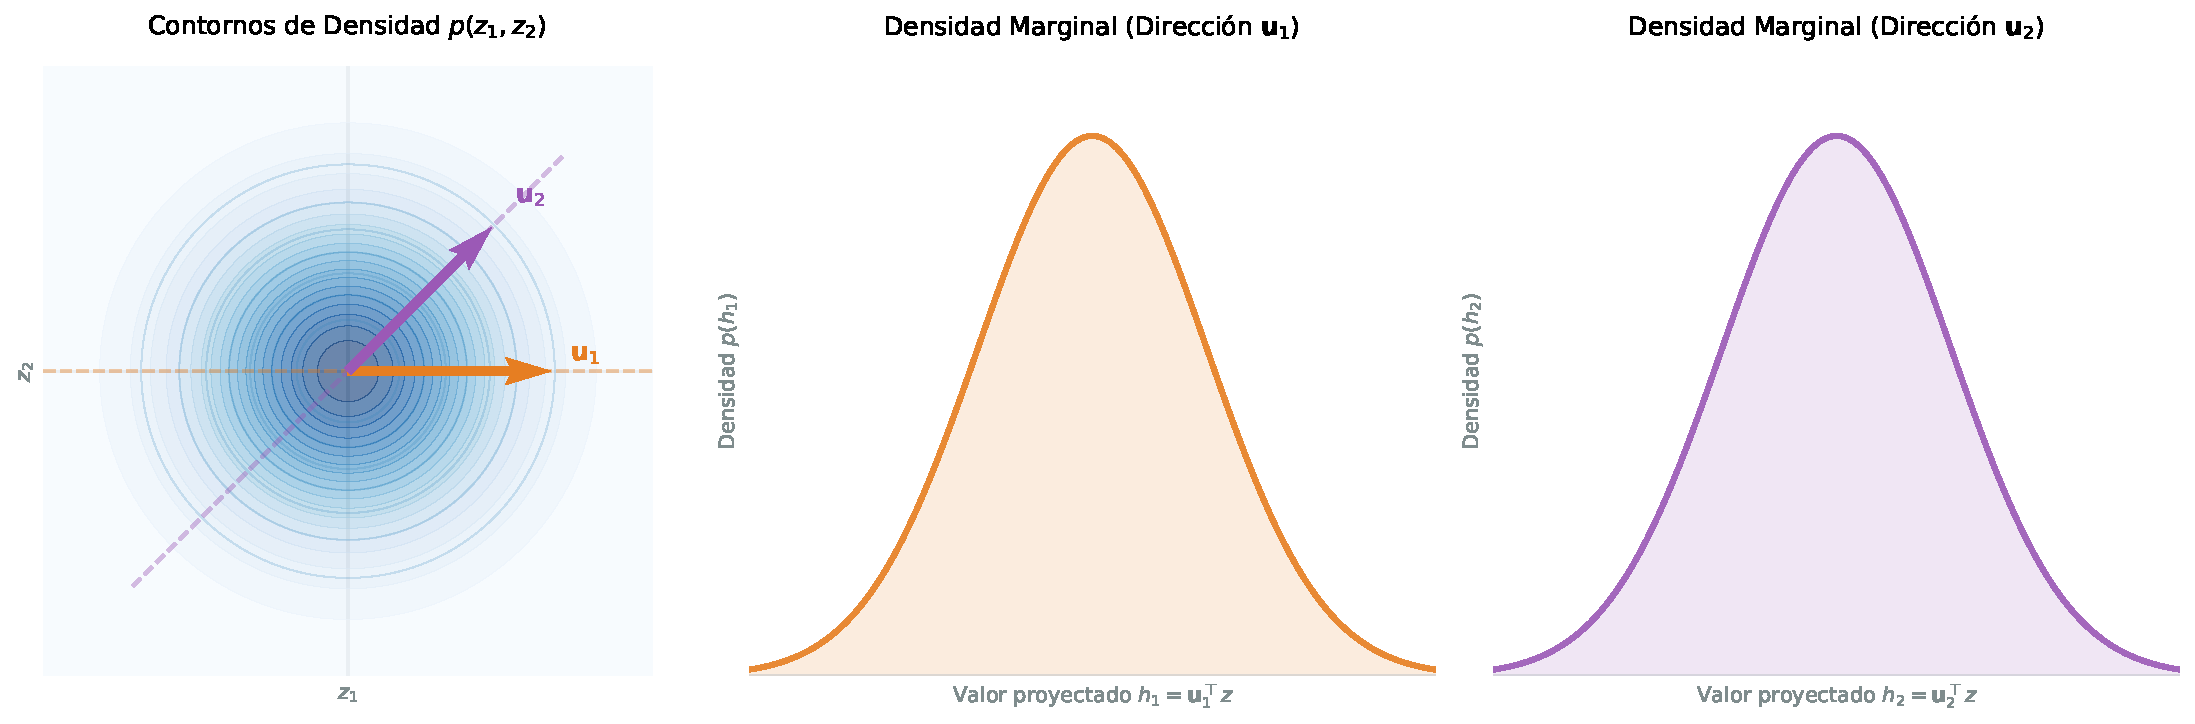
\includegraphics[width=0.95\linewidth, height=0.8\textheight, keepaspectratio]{cramer_wold.pdf}
\end{frame}

\begin{frame}{El Test de Epps-Pulley Diferenciable (1/2)}
Los test clásicos univariantes (e.g. Kolmogorov-Smirnov) emplean la operación de supremo ($\sup$) sobre la distribución acumulada empírica. Esto no es diferenciable y rompe el algoritmo de *backpropagation*.

Epps y Pulley (1983) formulan un test utilizando la Distancia $L^2$ sobre la \textbf{Función Característica} poblacional (la transformada de Fourier de la distribución).\footcite{epps1983test}
\end{frame}

\begin{frame}{El Test de Epps-Pulley Diferenciable (2/2)}
El estadístico resultante evalúa sobre la proyección muestral $h_1 \dots h_n$:
\[
    T_{EP}(\mathbf{h}) = 1 + \frac{\sqrt{2}}{n^2} \sum_{j,k} e^{-\frac{(h_j - h_k)^2}{4}} - \frac{4}{\sqrt{3}\, n} \sum_{j} e^{-\frac{h_j^2}{6}}
\]

Esta formulación analítica exacta es una suma finita de funciones exponenciales, lo que la hace de clase $\mathcal{C}^\infty$ e \textbf{infinitamente diferenciable} respecto de las observaciones, integrándose a la perfección en redes neuronales.
\end{frame}

\begin{frame}{SIGReg y LeWorldModel}
La pérdida total que rige el entrenamiento del LeWorldModel condensa toda la corrección:
\[
    \mathcal{L}_{\text{LeWM}} = \mathcal{L}_{\text{pred}} + \lambda\, \text{SIGReg}(Z)
\]
donde $\text{SIGReg}(Z) = \frac{1}{M} \sum_{m} T_{EP}(Z\mathbf{u}^{(m)})$.

Esta formulación elegante reemplaza 7 términos en PLDM por solo 1 término probabilístico exacto, eliminando gradientes contradictorios y forzando explícitamente el Puente de Jaynes sin negativos.
\end{frame}

\begin{frame}{SIGReg en LeWorldModel}
\centering
\resizebox{!}{0.8\textheight}{%
\begin{tikzpicture}[
    node distance=1.5cm,
    inputbox/.style={draw, rectangle, rounded corners, minimum width=2.2cm, minimum height=0.8cm, align=center, fill=gray!5, font=\footnotesize\sffamily},
    matbox/.style={draw, rectangle, rounded corners, minimum width=2.2cm, minimum height=1cm, align=center, fill=gray!5, font=\footnotesize\sffamily},
    termbox/.style={draw, rectangle, rounded corners, minimum width=2.5cm, minimum height=1cm, align=center, font=\footnotesize\bfseries},
    arrow/.style={->, >=stealth, thick, rounded corners},
    operator/.style={draw, circle, fill=gray!10, font=\footnotesize\bfseries, inner sep=2pt}
]

% SIGReg Branch
\node[termbox, fill=blue!10, draw=black] (l_sigreg) at (0, 0) {$\text{SIGReg}(Z)$};

\node[operator, fill=gray!10, draw=black] (avg) at (0, 1.2) {$\frac{1}{M} \sum$};
\draw[arrow] (avg.south) -- (l_sigreg.north);

\node[matbox, fill=orange!10, draw=orange!50] (ep1) at (-2.0, 2.5) {Epps-Pulley\\$T(\mathbf{h}^{(1)})$};
\node[matbox, fill=purple!10, draw=purple!50] (epM) at (2.0, 2.5) {Epps-Pulley\\$T(\mathbf{h}^{(M)})$};
\node[font=\footnotesize\bfseries] (dots) at (0, 2.5) {$\dots$};

\draw[arrow, orange] (ep1.south) |- (avg.west);
\draw[arrow, purple] (epM.south) |- (avg.east);

% CW Box
\node[draw=blue!30, dashed, rounded corners, fill=blue!2, inner sep=10pt, minimum width=7.5cm, minimum height=2.8cm] (cw_box) at (0, 5.0) {};
\node[font=\footnotesize\bfseries, text=blue!80] at (-1.0, 6.0) {Cramér-Wold (Proyecciones)};

\node[align=left, font=\scriptsize] (uM) at (-2.5, 5.4) {$\mathbf{h}^{(M)} = Z \mathbf{u}^{(M)}$};
\node[font=\scriptsize] at (-2.5, 4.8) {$\vdots$};
\node[align=left, font=\scriptsize] (u1) at (-2.5, 4.2) {$\mathbf{h}^{(1)} = Z \mathbf{u}^{(1)}$};

\node[inner sep=0pt] at (1.5, 4.8) {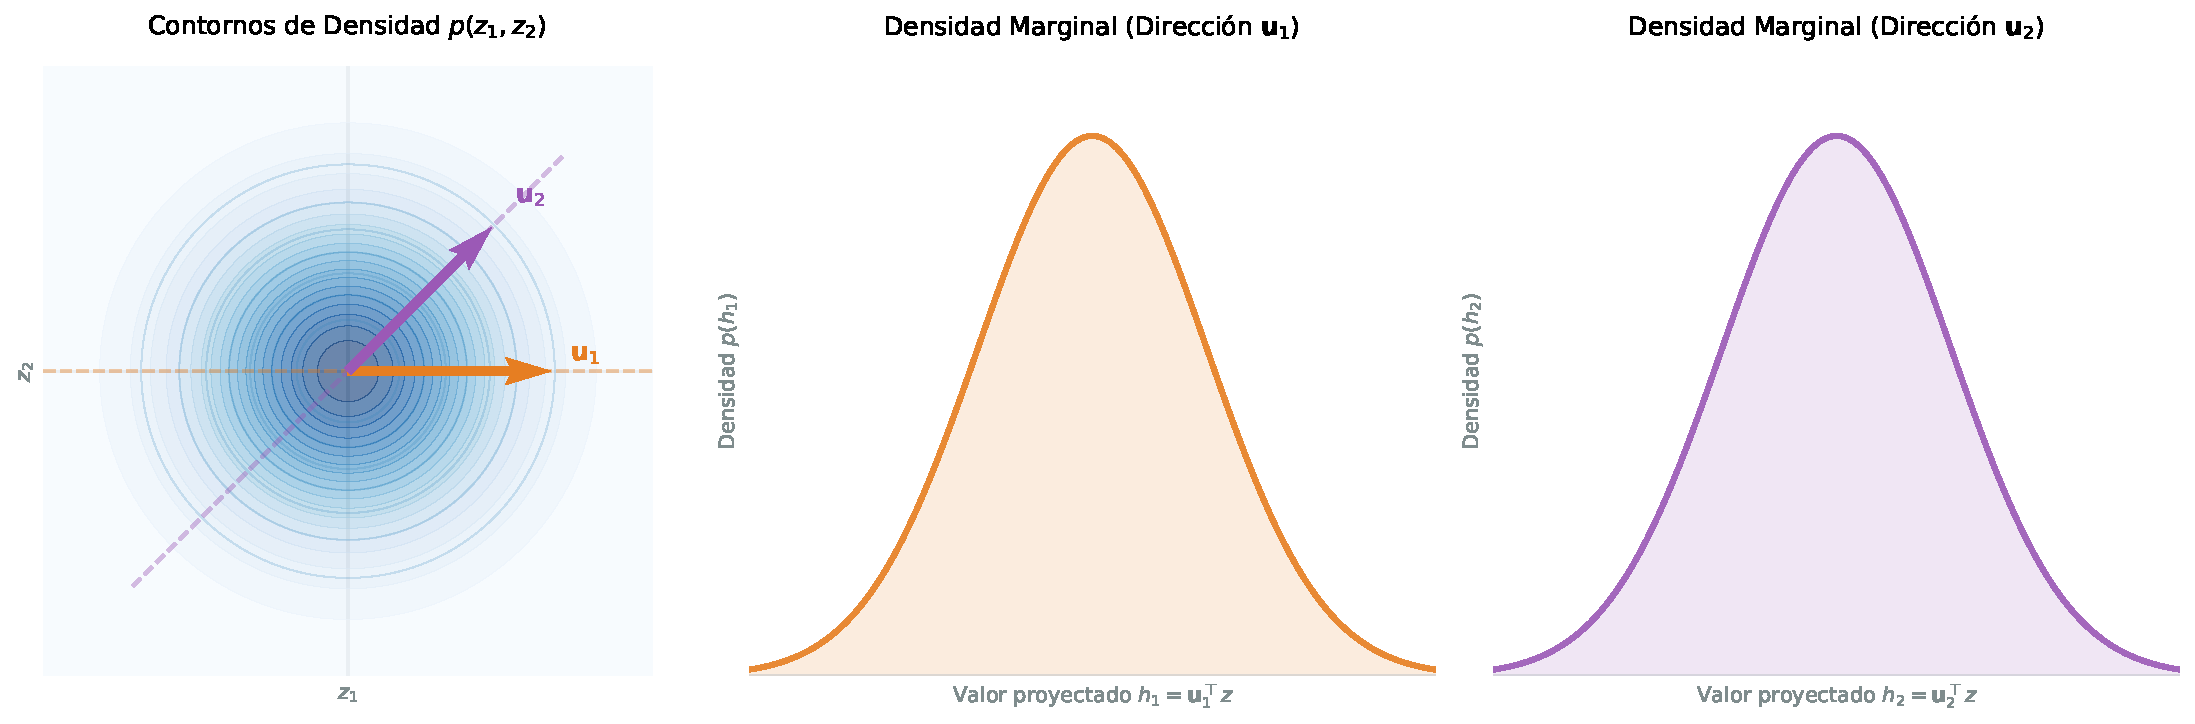
\includegraphics[width=3.5cm, keepaspectratio]{cramer_wold.pdf}};

\draw[arrow, orange] (-2.0, 3.6) -- (ep1.north);
\draw[arrow, purple] (2.0, 3.6) -- (epM.north);

\node[inputbox] (z_all) at (0, 7.2) {Representaciones\\$Z \in \mathbb{R}^{B \times d}$};
\draw[arrow] (z_all.south) -- (cw_box.north);

% Background Groups
\begin{scope}[on background layer]
    \node[draw=gray, dashed, rounded corners, fit=(z_all)(cw_box)(ep1)(epM)(l_sigreg), inner sep=10pt, fill=gray!3] (sigreg_bg) {};
    \node[anchor=south, font=\footnotesize\bfseries, text=gray!60] at (sigreg_bg.north) {$\mathcal{L}_\text{SIGReg}$};
\end{scope}
\end{tikzpicture}%
}
\end{frame}

\begin{frame}{El Arco Narrativo y Cierre de Barlow}
\centering
\resizebox{0.95\linewidth}{!}{%
\begin{tikzpicture}[
    node distance=0.5cm,
    problem/.style={draw=red!70!black, rounded corners, minimum width=2cm, minimum height=1.2cm, align=center, fill=red!8, font=\scriptsize, text=black},
    solution/.style={draw=blue!70!black, rounded corners, minimum width=2cm, minimum height=1.2cm, align=center, fill=blue!8, font=\scriptsize, text=black},
    assumption/.style={draw=yellow!70!black, rounded corners, minimum width=2cm, minimum height=1.2cm, align=center, fill=yellow!10, font=\scriptsize, text=black},
    final/.style={draw=green!60!black, rounded corners, minimum width=2cm, minimum height=1.2cm, align=center, fill=green!10, font=\scriptsize, thick, text=black},
    arrow/.style={->, >=stealth, thick, gray!70},
    label/.style={font=\tiny, text=black, align=center}
]
% Nodos
\node[problem] (collapse) {Colapso\\Trivial y\\Dimensional};
\node[label, above=0.1cm of collapse] {Cap.~3\\(1993)};
\node[solution, right=of collapse] (contrastive) {P\'{e}rdidas\\Contrastivas\\$\mathcal{L}_{\text{neg}}$};
\node[label, above=0.1cm of contrastive] {Cap.~4\\(2006)};
\node[problem, right=of contrastive] (exp) {Escala\\exponencial\\$\mathcal{O}(e^d)$};
\node[solution, right=of exp] (barlow) {Barlow Twins\\VICReg\\(decorrelaci\'{o}n)};
\node[label, above=0.1cm of barlow] {Cap.~5\\(2021--2022)};
\node[assumption, right=of barlow] (gauss) {Hip\'{o}tesis\\Gaussiana\\no verificada};
\node[solution, right=of gauss] (jepa) {V-JEPA\\(heur\'{i}sticas\\ad-hoc)};
\node[label, above=0.1cm of jepa] {Cap.~6\\(2022--2025)};
\node[final, right=of jepa] (sigreg) {\textbf{SIGReg}\\Normalidad\\forzada};
\node[label, above=0.1cm of sigreg] {Cap.~7\\(2025--2026)};
% Flechas
\draw[arrow] (collapse) -- (contrastive);
\draw[arrow] (contrastive) -- (exp);
\draw[arrow] (exp) -- (barlow);
\draw[arrow] (barlow) -- (gauss);
\draw[arrow] (gauss) -- (jepa);
\draw[arrow] (jepa) -- (sigreg);
% Arco de cierre
\draw[->, >=stealth, thick, green!50!black, dashed] (sigreg.south) to[out=-90, in=-90, looseness=0.5] node[below, font=\scriptsize\itshape, text=green!50!black, yshift=-0.1cm] {Cierre del Principio de Barlow} (barlow.south);
% Leyenda
\node[below=1.8cm of collapse, font=\scriptsize, anchor=west] (leg) {
    {\tikz\draw[fill=red!8, draw=red!70!black, rounded corners] (0,0) rectangle (0.4,0.25);} Problema \quad
    {\tikz\draw[fill=blue!8, draw=blue!70!black, rounded corners] (0,0) rectangle (0.4,0.25);} Soluci\'{o}n \quad
    {\tikz\draw[fill=yellow!10, draw=yellow!70!black, rounded corners] (0,0) rectangle (0.4,0.25);} Hip\'{o}tesis pendiente \quad
    {\tikz\draw[fill=green!10, draw=green!60!black, rounded corners] (0,0) rectangle (0.4,0.25);} Resoluci\'{o}n final
};
\end{tikzpicture}%
}
\end{frame}

% ────────────────────────────────────────────────────────────
\section{Conclusiones y Líneas Futuras}

\begin{frame}{Conclusiones (1/2)}
\begin{enumerate}
  \item \textbf{EBMs como marco unificador:} formalizan la compatibilidad sin requerir probabilidad. La constante de normalización obliga a operar de manera no paramétrica.
  \item \textbf{El colapso como hilo conductor:} el aprendizaje JEA es una sucesión continua de soluciones analíticas y topológicas para evadir la degeneración latente.
\end{enumerate}
\end{frame}

\begin{frame}{Conclusiones (2/2)}
\begin{enumerate}
  \setcounter{enumi}{2}
  \item \textbf{El cierre de Barlow:} SIGReg impone explícitamente que $Z$ asuma una distribución normal isótropa, independizando dimensiones sin requerir heurísticas.
  \item \textbf{Recuperación Garantizada:} Klindt et al. (2026) demostraron formalmente que la gaussiana isótropa de SIGReg es la única formulación que asegura la recuperación lineal (ICA) de las verdaderas variables físicas del entorno subyacente.\footcite{klindt2026lejepa}
\end{enumerate}
\end{frame}

\begin{frame}{Líneas futuras}
\textbf{H-JEPA y Predicción Jerárquica:}
Los modelos temporalmente planos (1-step) fallan en horizontes largos de planificación (Control Robótico). Integrar SIGReg en estructuras jerárquicas con abstracción temporal multinivel es investigación de frontera.

\vspace{0.8cm}
\textbf{Sistemas dinámicos observacionales complejos:}
Llevar estas arquitecturas más allá de la robótica visual a tareas analíticas con simuladores latentes: estimación de modelos fluidodinámicos, diseño biomédico o ingeniería de materiales.
\end{frame}

\begin{frame}[plain]
\vfill
\centering
{\Large\bfseries\color{USred} Gracias por su atención}

\vspace{1cm}
{\large\itshape ``Las redes convolucionales de LeCun, formuladas en los ochenta,\\
esperaron casi cuatro décadas hasta que la escala computacional\\
les dio la razón. ¿Será el destino de las JEA repetir esa trayectoria?''}

\vspace{1cm}
{\normalsize Pedro Rivas Vega\\
\texttt{Grado en Matemáticas — Universidad de Sevilla}\\
Julio 2026}
\vfill
\end{frame}

\begin{frame}[allowframebreaks]{Referencias}
\printbibliography[heading=none]
\end{frame}

\end{document}
